SMCube\cite{smcube} è un tool per la modellazione, simulazione e generazione di codice per automi a stati finiti (\textsl{ASF}) a tempo discreto. È stato progettato per essere integrato all'interno di \textit{Scicos}\cite{scicos}, permettendo la creazione di data-flow diagram che contengono ASF. In questo modello ibrido, i componenti del data-flow diagram vengono usati per gestire il flusso dei dati, mentre gli automi a stati finiti vengono usati per aggiungere comportamenti più complessi, non facilmente implementabili altrimenti.

A livello applicativo, l'integrazione di ASF progettati con SMCube all'interno di diagrammi Scicos è molto semplice: è sufficiente inserire un blocco SMCube all'interno del diagramma e specificare il file in cui è stato definito l'automa a cui il blocco si riferisce, come mostrato in figura \ref{Fig:smcube_ex}.

\begin{figure}
\centering
\makebox[\textwidth][c]{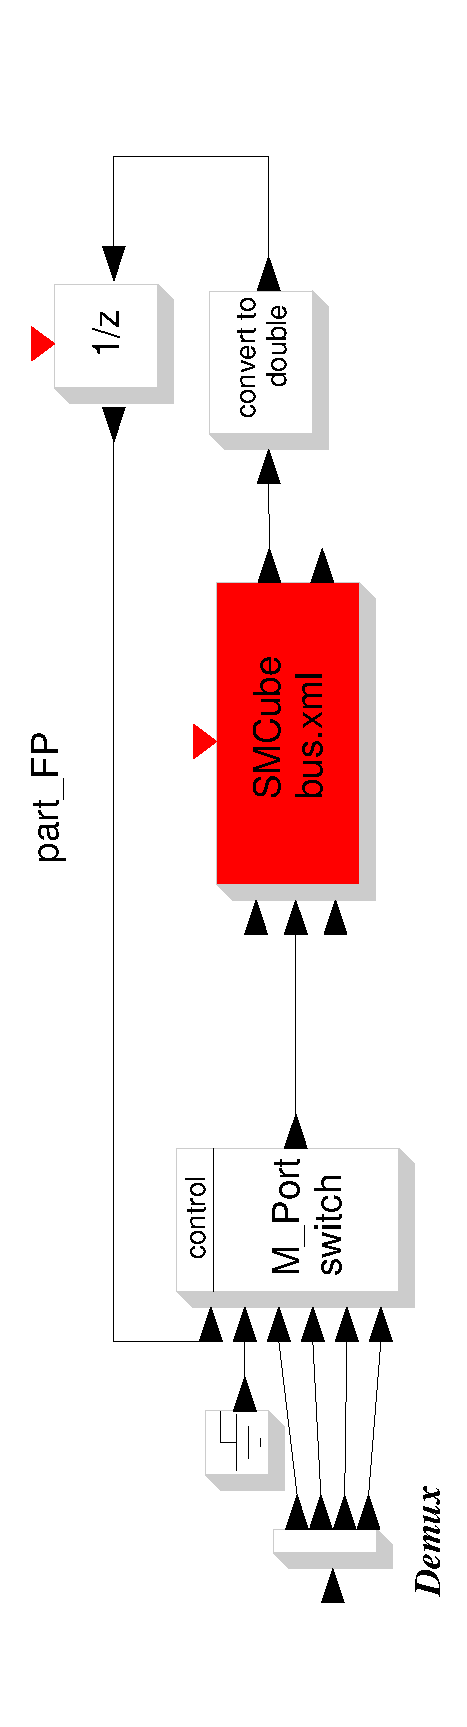
\includegraphics[angle=-90, width=1.2\textwidth]{smcube_block_ex.eps}}%
\caption{Blocco SMCube (in rosso) all'interno di un diagramma Scicos.}
\label{Fig:smcube_ex}
\end{figure}